\label{subsec:case_studies}

\colin{How often did we have to back up?}

\begin{table*}
\centering
\begin{tabular}{l|l|l|l|l}
Bug Name & Topology & Replay Success Rate & Total Inputs & MCS Size \\
\hline
POX list removal & 2 switch mesh & 20/20 & 69 & 2 \\
% With DP events: 72/2
% Original: config/eugene_epsilon_replay.py
% MCS: config/eugene_epsilon_mcs.py
POX in-flight blackhole & 2 switch mesh & 15/20 [20/20*] & 26 & 11 \\
% With DP events: 68/25
% Original: 7ba95ed82ca4e32f12ab511d9c4301dbac2c59d5
% MCS: 399cf861db87a65e600283d9ae7760400c4676e2
% Updated: updated_debug_branch_loop/
POX migration blackhole & 4 switch mesh & 20/20* & 29 & 3 \\
% With DP events: 117/3
% fuzz_pox_4mesh_blackhole
% Updated (fat tree): pox_fattree_migration
NOX discovery loop & 4 switch mesh & 18/20 & 150 & 18 \\
% With DP events: 358/58
% Original: ce547fc1df3bde279b6f3dd589c909663e295f1e
% MCS: 5f49e791b0c1a611454cf0930f54aa609dd635d3
% Updated to new format: nox_mesh_4_loop
Floodlight loop & 3 switch mesh & 15/50 & 284 & 36 \\
% Andi
\end{tabular}
\caption{Overview of Case Studies. \newline
\textmd{*with multiplexed sockets, overridden {\tt gettimeofday()}, and
logging interposition enabled.}}
\label{tab:case_studies}
\end{table*}

We have applied \projectname~to three open source SDN control platforms:
POX~\cite{pox}, NOX~\cite{nox}, and Floodlight~\cite{bigswitch}. Over a span
of roughly five days of
investigation we found a total of five bugs. We show a high-level overview
of our results in Table~\ref{tab:case_studies}, and
illustrate in detail how \simulator~found their minimal causal sequences
in the rest of this section. Interactive visualizations and replayable event traces
for all of these case studies are available at
\href{http://ucb-sts.github.com/experiments}{ucb-sts.github.com/experiments}.

\subsection{POX List Removal}
The first SDN control platform we examined was POX, the successor of NOX. POX is
a single-machine control platform intended primarily for research prototyping
and educational use (\ie~not large scale production use). Nevertheless, POX has
been deployed on real networks, and has a growing set of users.

The POX application we ran was a layer two routing module (`l2\_multi') that
learns host locations and installs exact match per-flow paths between known hosts using a variant of the
Floyd-Warshall algorithm. It depends on a discovery module, which sends
LLDP packets to discovery links in the network, and a spanning tree module,
which configures switches to only flood packets for unknown hosts along a
spanning tree.

We start with a relatively trivial bug to illustrate that
\projectname~is useful for early stage development and testing.
We employed \projectname~to generate random sequences of
inputs, and found after some time that POX threw an exception due to
attempting to remove an element from a list where the element was not present.

There were $69$ randomly generated inputs in the trace leading up to the
exception. We invoked \simulator~to identify a two element MCS:
a failure of a connected switch followed by a reboot/initialization of the same switch.
The nearly logarithmic runtime
behavior of \simulator~for this case is shown in Figure~\ref{fig:list_runtime}.

\begin{figure}[t]
    %\hspace{-10pt}
    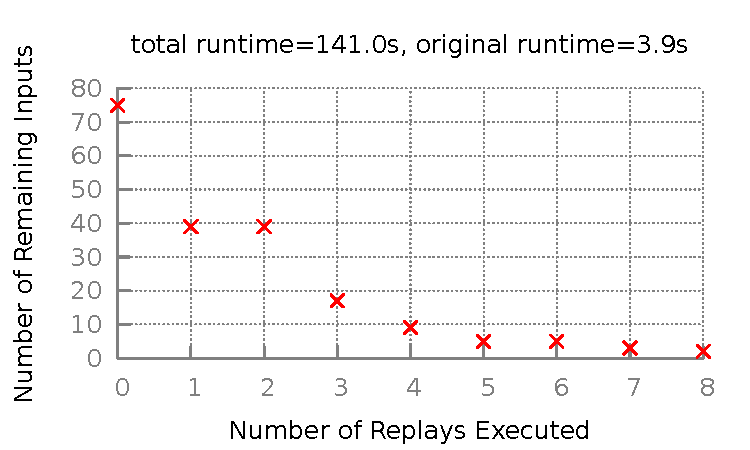
\includegraphics[width=3.25in]{../graphs/runtime/list_remove_error.pdf}
    \caption[]{\label{fig:list_runtime} Minimizing the POX list remove trace.}
\end{figure}

Apparently the developers of POX had not anticipated this particular event
sequence. Given the rarity of switch recovery events, and the tediousness of
writing unit tests for scenarios such as this
(which involved multiple OpenFlow initialization handshakes), this is not
surprising.
%Consider that the state-of-the-art open source technology for prototyping SDN
%applications, Mininet~\cite{handigol2012reproducible}, excels at
%testing common scenarios (on production OpenFlow software switches),
%but is not explicitly designed for scripting corner-case scenarios such as
%switch failure/recovery.
\projectname~made it straightforward to inject inputs
at a high semantic level,
and the minimized event
trace it produced made for a simple integration test.

%We illustrate type errors to show how STS is a useful framework for exploring
%code paths that you forget to unit tests.

\subsection{POX In-flight Blackhole}
We discovered the next bug after roughly 20 runs of randomly generated inputs.
We noticed that \projectname~reported a persistent blackhole while POX was bootstrapping its
discovery of link and host locations. We encountered this bug
on a simple topology, depicted in Figure~\ref{fig:simple_topo}, consisting of
two hosts A and B
and two switches S1 and S2 connected by a single link.

\begin{figure}[t]
    %\hspace{-10pt}
    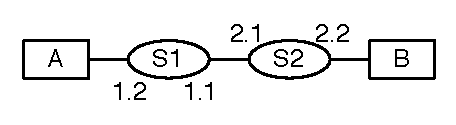
\includegraphics[width=3.25in]{../diagrams/state_machines/mesh_topo.pdf}
    \caption[]{\label{fig:simple_topo} Topology for POX
    in-flight blackhole. Numbers denote port labels.}
\end{figure}

There were $29$ inputs in the initial trace, and \simulator~returned a $11$ input
MCS (runtime shown in Figure~\ref{fig:pox_discovery}). With the MCS in hand we took out paper and pencil to decipher what had
transpired.

\begin{figure}[t]
    %\hspace{-10pt}
    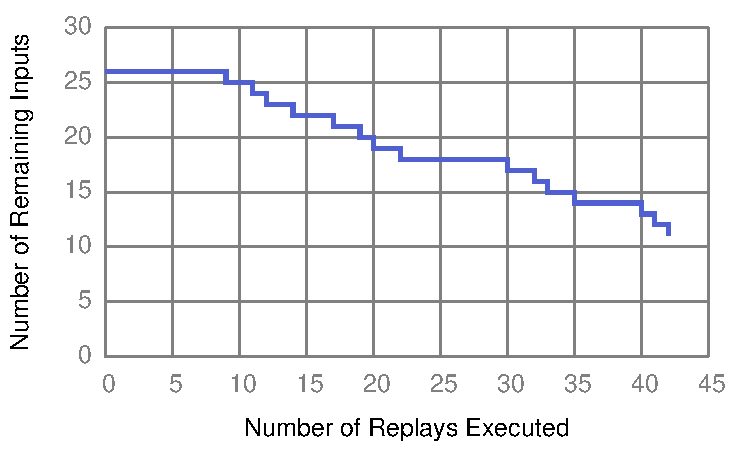
\includegraphics[width=3.25in]{../graphs/runtime/pox_blackhole.pdf}
    \caption[]{\label{fig:pox_discovery} Minimizing the POX in-flight blackhole.}
\end{figure}

Before the discovery module had learned of the link connecting the two
switches,
there were six traffic injection events between hosts (A$\rightarrow$ B and
B$\rightarrow$A). At the point when the link was discovered, POX had
previously learned
of B's location at port $2.2$, and correctly unlearned a previous location for
A at port $2.1$ (which it now knew to be a switch-switch link). %Upon POX would oscillate between learning the correct location
%of hosts at their ingress switch, and then learning an incorrect location
%when the flooded packet traversed the link and the next switch
%notified the controller of a new flow.\footnote{This seems to be necessary behavior before the
%links are discovered, since the hosts could have
%have legitimately migrated}
%This did not appear to be problematic though at first glance though,
%since we observed that POX correctly flushed the routing entries of the
%switches and forgot its incorrectly learned location of $A$ when it discovered
%that $1.1$ and $2.1$ were switch-switch ports, not host ports. At this point POX's only knowledge was the
%correct location of $B$ at $2.2$.

Directly after the link discovery we observed an {\em in-flight} packet arriving from A$\rightarrow$B at
port $2.1$
(without a prior flow notification from S1). This was POX's first error.
Upon examining the code, we found that it
did not account for in-flight packets concurrent with
link discovery. As a result,
POX incorrectly learned A's location at $2.1$, even though it knew that the link
could not have hosts attached. If the first packet had
instead originated at $1.1$, POX would not have made this mistake.

The next event we observed was another
{\em in-flight} packet from B$\rightarrow$A arriving at port
$1.1$. S1 notified POX of the unmatched flow, and POX appropriately printed a
log statement indicating that a packet had arrived at an internal switch port without a
previously installed flow entry. What happened next puzzled us though. POX
proceeded to install a path for this new B$\rightarrow$A flow, but the
path itself contained a loop: POX installed a B$\rightarrow$A entry going out both
$1.1\rightarrow2.1$ and $2.2\rightarrow2.1$, whereas it should have installed
only the latter (given A's current known location). The default behavior of
OpenFlow switches is to ignore matching route entries (with wildcarded in
ports) that forward out the
same port the packets arrived on. This is where we started observing the blackhole:
now whenever B sent traffic to A, it would be dropped at S1 until
the faulty routing entry would eventually expire $30$ seconds later.

We investigated the code that handled in-flight packets
arriving on switch-switch ports. The log statement that we had observed
earlier was inside a nested conditional, and the code for
installing the path was below and outside of the nested conditional conditional.
What struck us was that there was a commented out return statement directly
after the log statement. The comment above it read: ``Should flood instead of
dropping''. We tried reinserting the return statement and replaying, and
the blackhole ceased to appear.

In summary, we found that the crucial triggering events were two
in-flight packets (set in motion by prior traffic injection events):
POX incorrectly learned a host location as a result of the first in-flight
packet, and
failed to return out of a nested conditional as a result the second in-flight
packet. We have sent the replayable trace generated by \simulator~to the lead
developer of POX, and await his response. We suspect that these fine-grained race conditions had not
been triggered before because message timing in
Mininet~\cite{handigol2012reproducible} or real hardware is not
delayed arbitrarily as it was in \projectname.

%We suspect this race condition was not observed in Mininet because the rate at which we were sending packets was
%significantly slower than in Mininet (which also sends $ARP$ and
%$IPV6$ pings), so that there were no in-flight flow notifications to POX to
%correct the situation.
% Discussion of how our gizmos helped.

\subsection{POX Migration Blackhole}
Having examined the POX code in some depth, we noticed that there might be
some interesting corner cases related to host migrations.
We set up randomly generated inputs, included host
migrations this time, and checked for blackholes. Our initial input size was
$29$ inputs.
Before investigating the bug we
ran \simulator, and ended up with a $3$ input MCS (shown
in Figure~\ref{fig:pox_migration}): a packet injection from a
host A, followed
by a packet injection by a host B towards A, followed by a host migration of host A. This made it immediately
clear what the problem was. After learning the location of A and installing a
flow from B to A, the routing entries in the path were never removed after A
migrated, causing all traffic from B to A to blackhole until the routing
entries expired. We did not know it at the time, but this was a known problem,
and this particular routing module did not support host migrations. Nonetheless, this
case demonstrates how the MCS alone can point to the root cause.

\begin{figure}[t]
    %\hspace{-10pt}
    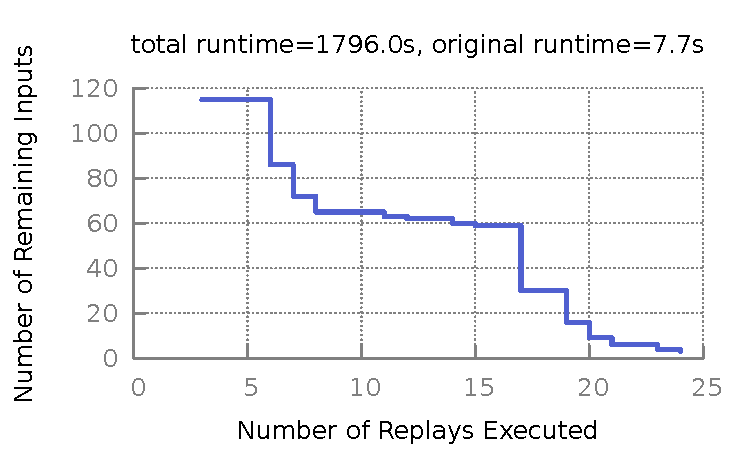
\includegraphics[width=3.25in]{../graphs/runtime/pox_migration_blackhole.pdf}
    \caption[]{\label{fig:pox_migration} Minimizing the POX migration
    blackhole.}
\end{figure}

\subsection{NOX Discovery Loop}

The next SDN control platform we examined
was NOX, the original OpenFlow controller.
NOX is also a single machine control platform, but unlike POX it has been used
fairly extensively in real networks.

Similar to POX we exercised NOX's routing module (`sprouting'), since
it draws in a large number of other components.
Routing learns link and host locations, installs all-to-all paths between
hosts on a per-flow basis, and is designed to be resilient to looped topologies.

We initially tested NOX on a two node topology, but did not find any immediate
problems. We then extended the topology to a four-node mesh, and discovered a
routing loop between two switches (involving routes for two hosts) within
roughly $20$ runs of randomly generated inputs.

Our initial input size was $150$ inputs, a minute's worth of execution.
\Simulator~returned a $18$ input MCS. The most salient inputs in the
MCS were $3$ dataplane packet drops mid-way through the execution, interspersed
with $14$ traffic injections. We are in the process of pinpointing the
exact root cause with NOX developers, based on the $18$ input MCS.

\begin{figure}[t]
    %\hspace{-10pt}
    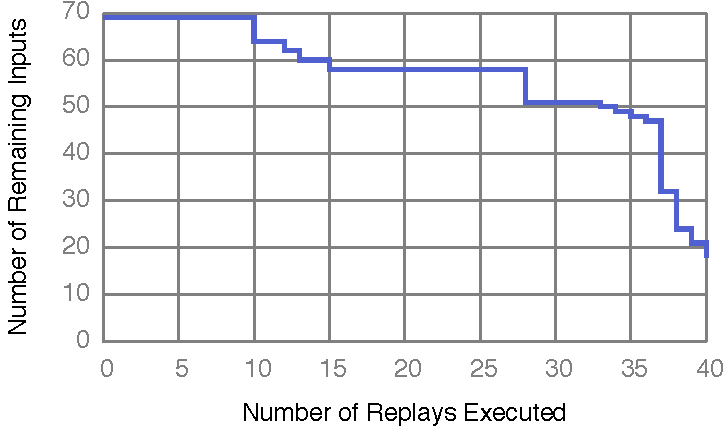
\includegraphics[width=3.25in]{../graphs/runtime/nox_loop.pdf}
    \caption[]{\label{fig:nox_discovery} Minimizing the NOX discovery loop.}
\end{figure}

\subsection{Floodlight discovery loop.}

We subjected the current (unmodified) open
source version of Floodlight (git commit f37046a) to fuzz testing with a three
node fully meshed topology and high failure event rates. In an hour-long experiment,
the fuzzer found an event sequence with $284$ total events
that results in a 3-node forwarding loop.

Floodlight makes use of multiple kernel level
threads, and thus can exhibit non-deterministic behavior.
Thus, it is not surprising that we do not achieve full reproducibility of this
bug during replay without further instrumentation. On average, 15/50 (30\%) of
replays reproduce the bug. To proceed with MCS isolation, we replayed the
execution up to 13 replays for each subsequence chosen by delta debugging. Statistically, this enables
STS to correctly diagnose violations in >99\% of cases.\footnote{$ln( 1 -
0.99) / ln( 1 - 0.30) \approx 13$}

\Simulator~was able to reduce the number of input events to $36$ input events.
Comparing output traces of successful and
unsuccessful runs, we noticed that the bug seems to correlate with specific
thread level race conditions between state updates in the \emph{LinkDiscovery} module and
the \emph{Forwarding} module. We are in the process of investigating the actual root cause.

This experiment provides a baseline for a worst case scenario of our system.
\projectname~exercised an unmodified, multithreaded controller that it does
not have deterministic control over.
The bug appears to depend on fine-grained thread-level races
conditions that are difficult to guarantee. Still, \projectname was instrumental
in pointing out a previously unknown bug, and reducing the input size.

\noindent{\bf Overall Results.} The overall results of our case studies are
shown in Table~\ref{tab:case_studies}.
We show the initial input size and MCS input size in the last two columns.
For the Replay Success Rate column we
repeatedly replayed the original unpruned event trace, and measured how often we
were able to reproduce the policy violation. There was indeed non-determinism
in some cases, especially Floodlight. For the specific case of
POX in-flight blackhole, we were able to eliminate the relevant
non-determinism by employing multiplexed sockets, overriding {\tt
gettimeofday()}, and waiting on
POX's logging messages. We expect that we would see similar improvements if we
applied these techniques to Floodlight.

We measured the runtime of \simulator~for these case studies in Figures $6 \& 8--11$.
While some instances ran in logarithmic time, the worst case was minimizing NOX discovery loop,
which took more than $5.5$ hours. Nonetheless, we conjecture that even long iteration
sizes are often preferable to spending software developer's time on manual
diagnosis.

%\subsection{Overhead}
%
%Unlike traditional record and replay techniques, \projectname (at least in
%testing mode) does not incur
%Overhead: none! Logs already there. Deterministic replay on the other
%hand has a huge overhead.

%\subsection{Mitigating Non-Determinism}
%
%Our implementation of multiplexed sockets and
%Include how many lines it took to interpose on the logging library, and how
%many lines it took to answer snapshot requests.

%\subsection{New Internal Events}
%
%How often do unexpected internal events occur in practice?
% The logging statements must also contain enough context[d] to allow for
% unambiguous fingerprinting. -> what exactly this means

\subsection{Simulator Scalability}

Simulating networks in a single process potentially prevents \projectname~from
triggering bugs that only appear at large scale. We ran
\projectname~on large FatTree networks to see where these scaling limits lie.
On a machine with 6GB of memory, we booted POX as the controller, and measured the
time to create successively larger FatTree
topologies, complete the OpenFlow handshakes for each switch,
cut $5\%$ of links, and process POX's response to the link failures. As shown in
Figure~\ref{fig:scaling}, \projectname's processing time scales roughly
linearly up to $2464$ switches (a 45-pod FatTree). At that point, the machine
started thrashing, but this limitation could easily be removed by running an a
machine with more memory.

Note that \projectname~is not designed for simulating high-throughput dataplane
traffic; we only forward what is necessary to exercise the controller
software. In proactive SDN setups, dataplane events are not
relevant for the control software.

\begin{figure}[t]
    %\hspace{-10pt}
    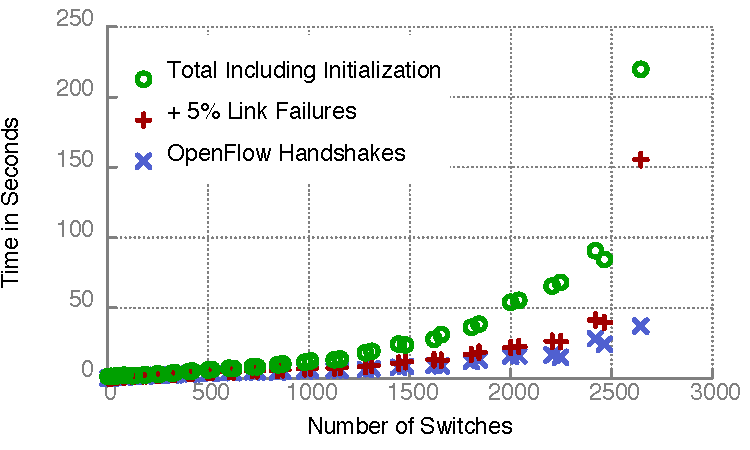
\includegraphics[width=3.25in]{../graphs/scalability/scaling.pdf}
    \caption[]{\label{fig:scaling} Simulation time for bootstrapping FatTree
    networks, cutting 5\% of links, and processing the controller's response.}
\end{figure}

\subsection{Parameters}
\label{subsec:params}

Our algorithm leaves an open question as to what value
\textepsilon~should be set to. We experimentally varied \textepsilon~on the
POX in-flight blackhole and the POX list removal bugs.
We found for both cases that the number of events we timed out on while isolating the MCS became stable for values above $25$ milliseconds.
For smaller values, the number of timed out events increased rapidly. We
currently set \textepsilon~to $100$ milliseconds.

\colin{Make me work}
%\begin{table*}
%\centering
%\begin{tabular}{l|l|l|l|l|l}
%Bug Name & \textepsilon & \textepsilon & \textepsilon & \textpsilon &
%\textepsilon \\
%\hline
%POX list removal (Replay) & 59.3\% & 98.0\% & 98.3\% & 98.3\% & 98.5\% \\
%POX list removal (MCS) & 58.3\% & 69.9\% & 69.9\% & 70.6\% & 70.9\% \\
%POX in-flight blackhole (Replay) & 24.4\% & 100.0\% & 100.0\% & 100.0\% & 100.0\% \\
%POX in-flight blackhole (MCS) & 24.0\% & 75.9\% & 75.9\% & 75.9\% & 75.2\% \\
%\end{tabular}
%\caption{Percentage of Events Matched for Values of \textepsilon in ms.}
%\label{tab:epsilon}
%\end{table*}

In general, larger values of \textepsilon~are preferable to
smaller values (disregarding runtime considerations), since we can always
detect when we have waited too long (\viz~when a successor of the next input
has occurred), but we cannot detect when we have timed out
early on an internal event that is in fact going to occur.
Analyzing event frequencies for particular bugs could provide more ideal
\textepsilon~values.


% ------------------------------------- %
%    OLD TEXT
\eat{

% Just realized: b/c of anonymity, the PC can't chastise us for
% running our system on our own code -- we can't tell them that it's our code!
We applied \projectname{} to three open source SDN control platforms:
Frenetic~\cite{frenetic}, POX~\cite{pox}, and Floodlight~\cite{bigswitch}, and
quickly found (or reproduced) one bug in each. The bug in Frenetic demonstrates
the utility of checking correspondence between high-level policies and
low-level configuration (without needing to specify invariants). The bugs in
POX and Floodlight demonstrate the importance of \simulator{}'s ability to
programmatically prioritize persistent correctness violations and infer their minimal
causal sets.

For all three cases, only a small code modification to the controller was necessary
to retrieve the platform's state for correspondence
checking.

\subsection{Case studies}

% Outline for bug reports:
%  - Describe each system under test
%  - Describe bugs found
%  - Lessons learned from finding bugs
Here we the discuss the three bugs we found with \projectname{}.

\noindent{\bf Frenetic.} Our first example is Frenetic~\cite{frenetic}, a control platform
providing functional-reactive language
support for programming OpenFlow networks.
Frenetic's language features aim to prevent common OpenFlow programming
errors such as race conditions and overlapping flow entries; Frenetic's
runtime system handles these low-level details on
the application's behalf. Frenetic is a modern SDN controller with a reactive
flow installation policy;
we present it here to demonstrate that \projectname{}, although focused
primarily on proactive controllers, can nonetheless be used to
troubleshoot errors in reactive control platforms.

When running learning switch, the simplest Frenetic application, we encountered
persistent correctness violations immediately. The propagation graph ($\Omega$) for Frenetic's
runtime representation of the network policy had leaves that were not present
in the physical network. Upon closer examination, we found that Frenetic's
runtime system was neglecting to remove old FLOOD routing entries from its
representation of the network policy after the hosts' route had been learned,
even though the learning switch application had
asked for these entries to be removed. Note that this case was not an overtly
malicious bug; the FLOOD entries had indeed been removed from the physical
network. The outdated controller state nevertheless went unnoticed; the bug in
Frenetic's runtime was not specific to the learning switch, and could have
resulted in failure to install flow entries at a later point in time if the
application had asked to re-install them. The key takeaway from this example
is that correspondence checking is a powerful mechanism for
verifying that the controller's representation of the network matches the true
network state correctly; without correspondence checking, troubleshooters
would need to compare the routing configurations and controller's data
structures side-by-side.

\noindent{\bf POX} Our second example is POX~\cite{pox}. POX is modeled after
Onix~\cite{onix}, a production SDN platform; as in Figure~\ref{fig:basicarch}
POX provides a physical view, a virtualized view, and a naive replication
mechanism between distributed control servers.

Because the functionality within POX is relatively young, we chose to
fabricate a bug in POX's distribution failover logic, and independently
validate that the simulator was able to identify, prioritize, and find the
minimal causal set for the fabricated correctness violation.

In particular, we injected the following bug: a controller replica performs
updates to switches by (i) updating the persistent datastore storing the state
of the network (thereby notifying other replicas of the update), and (ii) pushing the
update to the switch. A control server writes a new ACL entry update to the datastore, but crashes
before completing step (ii). The switch is adopted by a new replica,
but the new control server assumes that the state in the persistent datastore
is correct. The ACL entry is therefore never installed in the switch, and a
breach of tenant isolation occurs.

We interleaved this event sequence with a normal system execution trace, and
determined whether \simulator{} could identify the correctness violation.
Throughout the system execution there were a handful of transient
correctness violations overlapping with the isolation breach. Nonetheless, our
simulator was able to identify the correct correctness violation.

\noindent{\bf Floodlight: Distributed controller failover race condition}
We were able to reproduce the problem shown in Figure~\ref{fig:example} in our
simulation environment\footnote{The code is publicly available},
and apply \simulator{} successfully.
We modified the Floodlight software to provide an interface for extracting its
physical view. We did not interpose on internal events of the controller, but instead used a
heuristic to wait for $.5$ seconds between injecting inputs to allow the
controllers to fully react. We ran two of the modified Floodlight controller
instances, connected to two simulated switches, and injected 200 extraneous link
and switch failures, with the controller crash and switch connect event\footnote{We used a switch connect
event rather than a link failure event for logistical reasons, but both
can trigger the race condition} that triggered the blackhole interleaved among them.
On ten repeated runs, the algorithm successfully pruned all extraneous
inputs despite non-determinism in the Floodlight internal events. With full determinism and
interposition, we expect that the algorithm should work well for less
fabricated cases.

\subsection{Overhead}

\colin{Reviewer OB: I would prefer to see a more in-depth analysis of why
correspondence checking is not as heavyweight as, say, conventional
model-checking. Is it the inherent symmetry in data center networks? Can we
assume that there is symmetry?}

In addition to describing bugs, we show that \projectname{} is able
to simulate and check large networks quickly.

\noindent{\bf Record and Replay Overhead.} In contrast to general record-and-replay
mechanisms, the amount of recorded state needed for
high-fidelity replay is tractable. With proactive flow installation,
updates are pushed to routing tables over a relatively long time scale; periodic
FIB snapshots along with a log of link state events, control server
downtime, and host mobility information suffice for our purposes. As a point of reference, the Cisco 7000
core switch model supports a maximum of 128K MAC entries and
128K ACL entries~\cite{cisco7000}. Assuming 36 bytes per flow entry,
(larger than the OpenFlow 13-tuple), each FIB will contain a maximum of 9216
bytes, uncompressed. A datacenter of 100,000
hosts includes roughly 8,000
switches~\cite{Al-Fares:2008:SCD:1402958.1402967}.
Therefore a snapshot of the FIBs of the entire network takes up roughly 74 MB.
The VL2 paper reports 36M network error events over one year over 8
datacenters, which implies 8.5 error events per minute per
datacenter~\cite{Greenberg:2009:VSF:1592568.1592576}.
Suppose we took a snapshot of the FIBs in the network every second.
Then we would need to store roughly 4GB, uncompressed, per minute, a relatively small growth
rate for datacenter logs. This information, in addition to a log of host
mobility events (\eg{} VM migrations) will suffice for our purposes. Note that this is a conservative overestimate.

\colin{Notes from Rean Griffith:
\begin{itemize}
\item total vms in a typical datacenter: 1000
\item migration frequency (migrations/minute): 20 per hour
\item VM spin ups/downs: 150 power ons per hour (see our OSR 2010 paper for
power off estimates)
\item Do we log VM migrations and how does that log grow (I wasn't able to
get any estimates on log-growth data)
\end{itemize}

We had an OSR 2010 paper that provided numbers scaled by the number of
VMs in an installation:
Challenges in building scalable virtualized datacenter management
(http://dl.acm.org/citation.cfm?id=1899941)
}

%To account for host mobility, assume that each server hosts 10 VMs,
%and 1\% of VMs are created, suspended, or migrated every minute. Then 10,000 host mobility events must be
%logged per minute, also a reasonable storage cost. \colin{get real numbers}

%As a point of reference, border routers' working RIB size is
%$\textasciitilde$130MB~\cite{Karpilovsky:2006:UFR:1368436.1368439}.

\noindent{\bf Correspondence Checking Runtime.} Computing the propagation
graph for correspondence checking is equivalent to enumerating
all possible paths in the network, which scales with the diameter
of the network and the number of routing entries per switch \colin{Reviewer
OC: scales how? I suspect it's at least N2}.
The propagation graph for each host can be
computed in parallel however, so the computation is bottlenecked by the serial runtime
of computing a single host's propagation graph.

We show the serial runtime of correspondence checking in
Figure~\ref{fig:hsa_runtime}. For this analysis we generated fat tree topologies
between 2 and 48 pods wide, with pre-installed PORTLAND~\cite{NiranjanMysore:2009:PSF:1592568.1592575}
routing tables in each switch. Each data point is the minimum of three
runs\colin{Reviewer OC: seems to overstate value of approach if maximum is much different} on a single Intel Xeon 2.80GHz core. Note that the number of PORTLAND routing entries per switch scales with the number
of pods in the fat-tree. We excluded the time to convert
flow tables to HSA transfer functions, since transfer functions can be maintained
offline.

\colin{Reviewer OB:  what are the characteristics of the PORTLAND routing
table? If the tables were any different, would the performance of
correspondence checking remain the same, degrade or improve? }

\colin{Reviewer OD: First the paper started generally, then it narrows its
scope to PORTLAND-style datacenters. An accurate abstract would have reflected
this narrowing of scope}

As the figure depicts, even for large networks
(27,648 hosts) the serial runtime of correspondence checking is reasonable for
interactive use. The number of serial tasks to be executed
is the number of hosts in the network squared, disregarding ECMP load balancing.
\colin{reviewer B: correspondence is not being checked. I should be clear
that this is the runtime of generating the propagation on the physical
network, which is an upper bound on the runtime of checking the virtual
network.}

\begin{figure}[t]
    %\hspace{-10pt}
    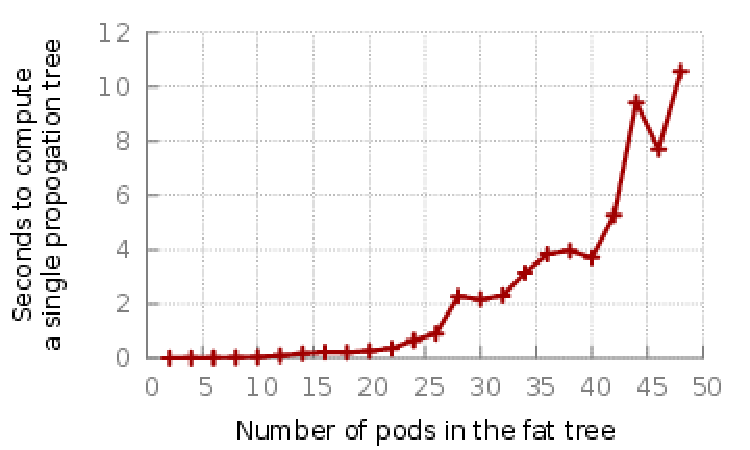
\includegraphics[width=3.25in]{../graphs/hsa_overhead_graph/graph.pdf}
    \caption[]{\label{fig:hsa_runtime} Serial runtime of correspondence
    checking on PORTLAND fat tree networks. Each datapoint consists of
    $x^3/4$ hosts and $5x^2/4$ switches (\eg{} 48 pods means 27,468 hosts
    attached to 2,880 switches)}
\end{figure}

\noindent{\bf Simulator Scalability.} Our design models the entire network
within a single process. We show in Figure~\ref{fig:scalability}
that this approach nonetheless scales to large networks. For this analysis we
generated fat tree topologies between 2 and 48 pods wide, where all switches in
the network connected to a single controller. The controller sent each switch
an OpenFlow
$FLOW\_MOD$ and subsequent $BARRIER\_REQUEST$ message, and waited for the
corresponding $BARRIER\_REPLY$. We then measured the time to between the first
$FLOW\_MOD$ sent and the last $BARRIER\_REPLY$ received. As expected, the
runtime was roughly linear with the number of switches in the network. The
figure also shows that the processing time for large networks (5 seconds per
simulator round) was well within the bounds for interactive use.

\begin{figure}[t]
    %\hspace{-10pt}
    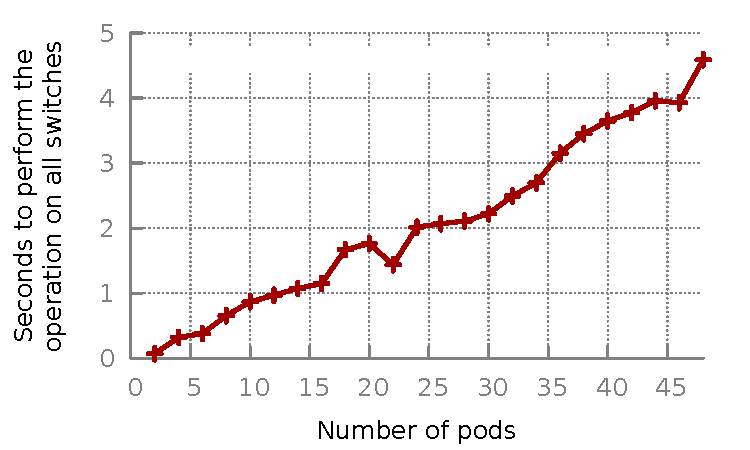
\includegraphics[width=3.25in]{../graphs/scalability_graph/scale.pdf}
    \caption[]{\label{fig:scalability} Time to send and process messages
    between controller and simulated switches. Each datapoint consists of
    $x^3/4$ hosts and $5x^2/4$ switches (\eg{} 48 pods means 27,468 hosts
    attached to 2,880 switches)}
\end{figure}

We also tested the extreme limits of the simulator's scalability, pushing up
the number of switches until something broke. We encountered what appears to be
a limitation of the Linux TCP/IP stack: TCP connection attempts began failing
beyond 26,680 sockets. Note that 26,680 switches is an order-of-magnitude larger than
the today's biggest networks.

\subsection{Replay fidelity}

On the one hand, since the SDN platform is in software, we can, in theory,
reproduce all software-induced policy violations (though not problems
resulting from flaky hardware implementing code incorrectly). However, this
requires setting up the simulator to emulate the appropriate conditions that
led to the policy violation, and that can be quite difficult. We hope to make
progress in this area along two dimensions.  First, we hope to help the
community build up a set of regression tests, so that a wide variety of
bug-triggering scenarios are available in a public repository. This would go a
long way towards providing adequate test coverage.

Second, we hope to gather error logs from real production deployments which
will help us populate this repository; this may require providing novel kinds
of anonymization, so that large datacenter operators would be willing to share
their problems (since they want their SDN code to work) without revealing the
details of their network.  This may require a infrastructural counterpart to
minimally-causal events; the smallest number of infrastructure components that
can reproduce the same bug.

Also, note that our correspondence checking algorithm can not verify
time-dependent policies such as ``No link should be congested more than 1\% of
the
time'', or ``No server should receive more than 500MB/s of external traffic''.
In future work we will extend our correspondence checking algorithm to
account for this class of policies.

\colin{reviewer B: in fact, in addition to temporal properties, the
correspondence checking algorithm cannot verify any properties involving
individual links since it only accounts for externally observable behavior!}
}
